% This is samplepaper.tex, a sample chapter demonstrating the
% LLNCS macro package for Springer Computer Science proceedings;
% Version 2.21 of 2022/01/12
%
\documentclass[runningheads]{llncs}
%
\usepackage[T1]{fontenc}
% T1 fonts will be used to generate the final print and online PDFs,
% so please use T1 fonts in your manuscript whenever possible.
% Other font encondings may result in incorrect characters.
%
\usepackage{graphicx}
% Used for displaying a sample figure. If possible, figure files should
% be included in EPS format.
%
% If you use the hyperref package, please uncomment the following two lines
% to display URLs in blue roman font according to Springer's eBook style:
%\usepackage{color}
%\renewcommand\UrlFont{\color{blue}\rmfamily}

\usepackage{hyperref}
\hypersetup{
    colorlinks=true,
    urlcolor=blue,
    linkcolor=black,
    citecolor=black,
    filecolor=black,      
    anchorcolor=black,
    pdftitle={Reverse Engineering Hyper-V},
    pdfauthor={Stefan-Octavian Radu},
}

% escape text in math mode
\usepackage{amsmath}

% multiple columns
\usepackage{multicol}
\setlength{\columnsep}{1.0cm}

% lst blocks
\usepackage{listings}
\newcommand{\cc}{\lstinline[mathescape]}
% Custom colors
\usepackage{xcolor}
\usepackage{realboxes}

% appendix title
\usepackage[titletoc]{appendix}

\definecolor{lstgreen}{rgb}{0,0.6,0}
\definecolor{lstgray}{rgb}{0.5,0.5,0.5}
\definecolor{lstgrayy}{rgb}{0.92,0.92,0.92}

\lstdefinestyle{mystyle}{
    backgroundcolor=\color{lstgrayy},
    commentstyle=\color{lstgreen},
    keywordstyle=\color{blue},
    numberstyle=\tiny\color{lstgray},
    stringstyle=\color{magenta},
    basicstyle=\ttfamily\footnotesize,
    captionpos=b,
    keepspaces=true,
    numbers=left,
    numbersep=5pt,
    showspaces=false,
    showtabs=false,
    tabsize=2,
    frame=lines,
    language=c,
    escapechar=|,
    breaklines=true,
}
\lstset{style=mystyle}

% missing math symbols
\usepackage{stmaryrd}

% set spacing between document and footnotes
\setlength{\skip\footins}{5mm}

% diacritics
\usepackage{fontspec}

%
\begin{document}
%
\title{On Reverse Engineering Hyper-V}
\subtitle{- Praktikum Report -}
%
%\titlerunning{Abbreviated paper title} If the paper title is too long for the
%running head, you can set an abbreviated paper title here
%
\author{Ștefan-Octavian Radu}
%
\authorrunning{S. Radu}
% First names are abbreviated in the running head. If there are more than two
% authors, 'et al.' is used.
%
\institute{Advisor: Lukas Beierlieb
\\Julius-Maximilians-Universität Würzburg 
\\Institute for Computer Science Chair for Computer Science II 
\\stefan.radu@stud-mail.uni-wuerzburg.de
\\\url{https://se.informatik.uni-wuerzburg.de/}}
%
\maketitle % typeset the header of the contribution
%

\keywords{Hyper-V
\and Reverse Engineering
\and Ghidra
\and QEMU/KVM
\and Windbg
}

\section{Introduction}

Hyper-V is the hypervisor solution shipped as part of the Windows operating
system. Guests running under Hyper-V can communicate with the hypervisor
through a calling mechanism similar to system calls (syscalls) in an operating
system. One would refer to such calls as \emph{hypercalls}. The Hypervisor Top
Level Functional Specification (TLFS) documents, among other things, the
functionality of the hypercall system and documents a number of hypercalls
\cite{tlfs}. However, being a closed-source system, not all hypercalls are
documented.

With the rising popularity of cloud solutions, securing the technologies that
the cloud is built upon is more relevant than ever. Our motivation for this
project is to contribute to the effort of security researchers who don't have
access to the source code of Hyper-V. By analysing the undocumented hypercalls
from Hyper-V, we can gain a better understanding of its inner workings, and
potentially find bugs which would compromise its security. We will present a
comprehensive description of a reverse engineering setup for Hyper-V running on
the GNU/Linux operating system. We will also exemplify the usage of this setup
by presenting our results from reverse engineering the
\cc{HvCallQueryNumaDistance} hypercall (number \cc{0x78}). 

\subsection{Lab Environment Specifications}

The analysis environment features an Intel Core i5-8250U CPU and 8GB of memory.
The operating system running is based on the \cc{6.7.6-arch1-1} version of the
Linux kernel. Linux is a particularly unusual choice for working on the
internals of the Windows operating system. We hope that presenting this setup
will prove useful to other researchers who prefer using the Linux operating
system. We will present our findings including shortcomings and roadblocks. The
target to be analysed is the \cc{hvix64.exe} executable, typically found in
\cc{C:\Windows\System32\hvix64.exe} on a machine running Windows. The version
of our binary file is \cc{10.0.19041.2006}.

\subsection{Outline} 

The remainder of this work is structured as follows. In Sections
\ref{sec:static} and \ref{sec:dynamic} we discuss the static and dynamic
analysis setup respectively. Section \ref{sec:findings} is comprised of our
findings regarding the \cc{0x78} hypercall. We end with conclusions in section
\ref{sec:conc}.

\section{Static Analysis Setup}
\label{sec:static}

In this section we will cover the setup we used for statically analysing the
Hyper-V hypercalls. In particular we will cover Ghidra \cite{ghidra}, a
powerful open-source disassembler and decompiler. We will mainly discuss
project setup and automation via scripting. We will briefly mention other
popular tools in the field of reverse engineering that could be used as
alternatives to Ghidra.

\subsection{Ghidra}

The main tool used for static analysis is Ghidra. Ghidra is a Software Reverse
Engineering (SRE) framework developed by the National Security Agency (NSA) of
the United States. Ghidra includes a fully featured set of tools for analysing
code compiled for a large variety of platforms, including Microsoft Windows.
From the tool set, the features which were most useful for analysing Hyper-V
include the powerful decompiler, the disassembler and the scripting interface
available as a Java or Python API \cite{ghidra}. Although its interface is dated
and not very intuitive to use, its feature set is very powerful.

Ghidra is distributed as Free and Open Source Software (FOSS) under the Apache
2.0 licence \cite{ghidra_license}. 

\subsection{Setup}

There are a number of useful steps which should be performed in order to more
easily work on reverse engineering Hyper-V's components. We took inspiration
from Microsoft's Introductory blog post on Hyper-V research, which has some
very insightful content, but is unfortunately geared towards IDA
\cite{intro_hyperv}.

Since we're running on a 64-bit Intel system, we will inspect the
\cc{hvix64.exe} \emph{Hypervisor 2.0} binary. Since we're running a GNU/Linux
system, we ran a Windows guest through the QEMU/KVM and pulled out the binary
from the virtualised environment.

For the start, we create a new Ghidra project, import the binary and open it with
the decompiler tool. \emph{Here be dragons!}

\vspace{-2mm}
\subsubsection{Useful Imports.}

Before starting to inspect the hypercall handlers' code, we can introduce some
helpful symbols into the Ghidra project. These include a number of important
structures, enums, or constants. To do this, we acquired the
\href{https://github.com/ionescu007/SimpleVisor/blob/master/vmx.h}{\cc{vmx.h}}
\footnote{\url{https://github.com/ionescu007/SimpleVisor/blob/master/vmx.h}}
and \href{https://github.com/ionescu007/hdk/blob/master/hvgdk.h}{\cc{hvgdk.h}}
\footnote{\url{https://github.com/ionescu007/hdk/blob/master/hvgdk.h}} header
files. To import the definitions into the Ghidra project we go to \cc{File}
$\to$ \cc{Parse C Source}, create a new \cc{Parse configuration} and add the
two headers in the list of \cc{Source files to parse}. We encountered a number
of errors on import, which could be fixed by adding missing definitions and
rewriting some macros as follows:

\vspace{-1mm}
\begin{itemize}
    \item add \cc{#define C_ASSERT(e) typedef char __C_ASSERT__[(e)?1:-1]} in
        \cc{vmx.h}
    \item add \cc{typedef unsigned short UINT16;} in \cc{hvgdk.h}
    \item add \cc{typedef __int64 UINT64;} in \cc{hvgdk.h}
    \item change each \cc{DECLSPEC(X)} to \cc{__declspec(align(X))} in \cc{hvgdk.h}
\end{itemize}

We expect the previously mentioned errors to not be raised on a Windows system.

\vspace{-2mm}
\subsubsection{Defining Types.}

We further defined a number of useful types directly related to the hypercalls,
such as the hypercall's structure and the hypercall enum group, among others.
This can be done through Ghidra's \emph{Data Type Manager}, which is typically
found in the lower left corner, or by going to \cc{Window} $\to$
\cc{Data Type Manager}. Some IDA PRO scripts, such as
\href{https://github.com/gerhart01/Hyper-V-scripts/blob/master/CreatemVmcallHandlersTable2016.py}{this
one}\footnote{\url{https://github.com/gerhart01/Hyper-V-scripts/blob/master/CreatemVmcallHandlersTable2016.py}},
served as reference for the data types. Figure \ref{fig:struct_editor} can be
inspected for a view of the Structure Editor.

\begin{figure}[h]
    \centering
    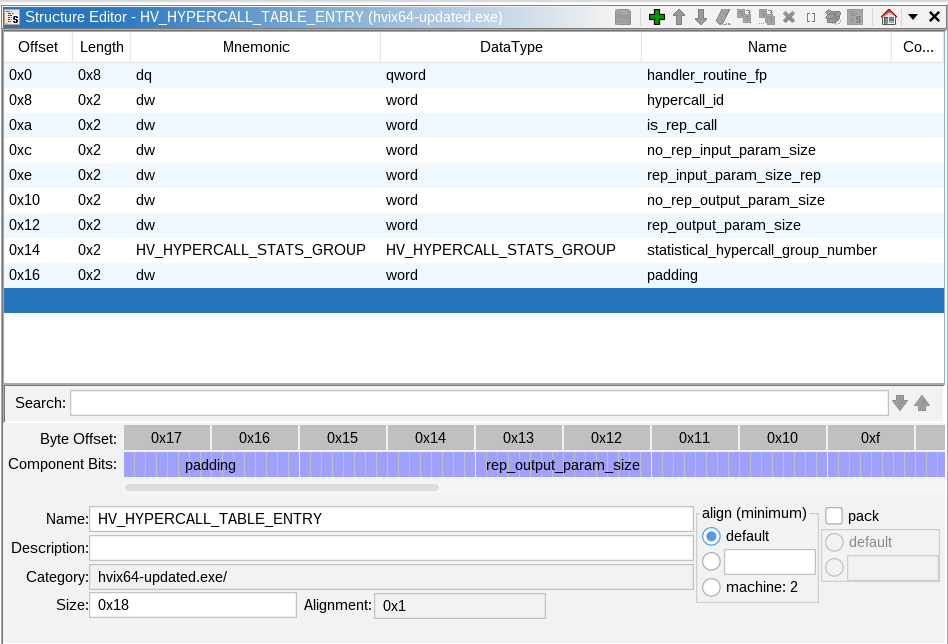
\includegraphics[width=0.85\textwidth]{./assets/struct.png}
    \caption{A view of the \cc{HV\_HYPERCALL\_TABLE\_ENTRY} struct, which we
    defined through the Ghidra structure Editor. We used it to retype each
    entry in the hypercall table from the \cc{CONST} section of the binary.}
    \label{fig:struct_editor}
\end{figure}

With the types defined, we can start retyping global variables. The first big
target is the hypercalls table from the \cc{CONST} section. We can manually set
the start address of the \cc{CONST} section to be of type
\cc{HV_HYPERCALL_TABLE_ENTRY[SIZE]}. At the type of writing, 260 hypercall
entries can be distinguished in the table. Each of the hypercalls returns
\cc{HV_STATUS}. Setting this return type for each available hypercall is very
useful during analysis. However, doing the type setting manually is time
consuming and impractical.

\vspace{-2mm}
\subsubsection{Scripting.}

Ghidra offers a scripting API in Java or Python for automating a wide array of
reverse engineering tasks. We can automate all the types creation and type
assignment by writing and running some Python scripts. Such scripts simplify
the setup process considerably. Listings \ref{lst:struct} and
\ref{lst:type_assign} exemplify data type creation and function signature
editing. The full scripts are available on
\href{https://github.com/Stefan-Radu/master/tree/master/an2_DE_erasmus/praktikum_hyperv_RE/hyper-v-ghidra-scripts}{github}\footnote{\url{https://github.com/Stefan-Radu/master/tree/master/an2_DE_erasmus/praktikum_hyperv_RE/hyper-v-ghidra-scripts}}.

\vspace{3mm}

\begin{lstlisting}[language=python, label={lst:struct},
    caption={Python script which creates the \cc{HV_HYPERCALL_TABLE_ENTRY} 
    structure.}]
struct = StructureDataType("HV_HYPERCALL_TABLE_ENTRY", 0)
struct.add(QWordDataType(), 8, "handler_routine_fp", "")
# similarly added field ...
struct.add(WordDataType(), 2, "rep_output_param_size", "")
dt_mgr = currentProgram.dataTypeManager
dt = dt_mgr.findDataType("/" + "HV_HYPERCALL_STATS_GROUP")
struct.add(dt, 2, "statistical_hypercall_group_number", "")
struct.add(WordDataType(), 2, "padding", "")
currentProgram.dataTypeManager.addDataType(struct, None)
\end{lstlisting}

\begin{lstlisting}[language=python, label={lst:type_assign},
    caption={Example of array creation and changing the name and return type
    of a hypercall function reference.}]
hvcalls_entry_type = dt_manager
    .findDataType("/HV_HYPERCALL_TABLE_ENTRY")
hvcall_entry_size = hvcalls_entry_type.getLength()
create_array_cmd = CreateArrayCmd(start_address,
    260, hvcalls_entry_type, hvcall_entry_size)
create_array_cmd.applyTo(currentProgram)

hvcall_ret_type = dt_manager.findDataType("/HV_STATUS")
hvcalls_entry_table = getDataAt(start_address)
entry = hvcalls_entry_table.getComponentAt(
    IDX * hvcall_entry_size)
hvcall_address = toAddr(entry.getComponent(0)
    .getValue().toString())
hvcall = getFunctionAt(hvcall_address)
hvcall.setName("HV_HYPERCALL_NAME", SourceType.ANALYSIS)
hvcall.setReturnType(hvcall_ret_type, SourceType.ANALYSIS)
\end{lstlisting}

A relevant note is that Ghidra is built in Java. The Python scripts run through
\cc{Jython}, which bridges the script code to the Java API. This adds an
obvious layer of overhead. Moreover, the python interface is based on
\cc{Python 2}, which is outdated. This, in turn, limits the usage of external
libraries. There are a number of plugins, such as \cite{ghidrathon}, which
address these issue, by introducing \cc{Python 3} scripting capabilities.

\vspace{-3mm}
\subsubsection{Result.}

After running the scripts, the \cc{CONST} section will be displayed in a more
intuitive and easy to work manner. As seen in Figures \ref{fig:const_before}
and \ref{fig:const_after}, we get a clearly defined table. Inspecting a 
hypercall handler's implementation can be done by clicking on the corresponding
field of an entry.

\begin{figure}
\centering
\begin{minipage}{.5\textwidth}
  \centering
  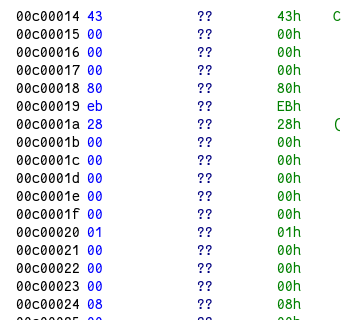
\includegraphics[width=0.88\linewidth]{./assets/const_before.png}
  \caption{The \cc{CONST} section before setup \\is displayed as a random
    array of bytes.}
  \label{fig:const_before}
\end{minipage}%
\begin{minipage}{.5\textwidth}
  \centering
  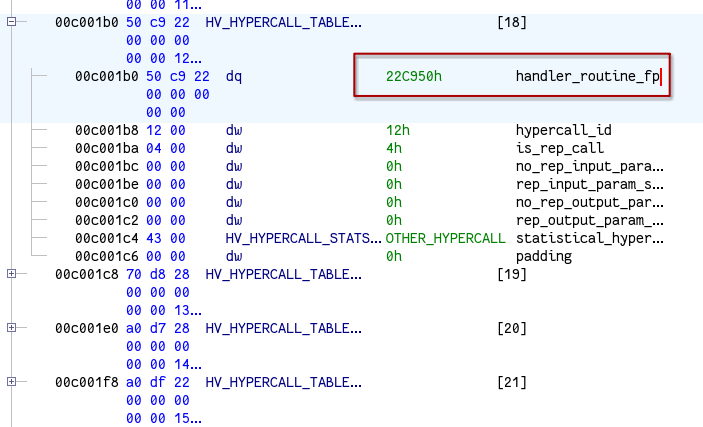
\includegraphics[width=0.98\linewidth]{./assets/const_after.png}
  \caption{After running the script, the \cc{CONST} section is displayed as
    an array. We can jump to any of the hypercall handlers' code by clicking on
    the \cc{handler_routine_fp} field of the corresponding entry.}
  \label{fig:const_after}
\end{minipage}
\end{figure}

\vspace{-5mm}
\subsubsection{Other Useful Features.}

Some other features that are by default hidden in Ghidra, but could prove
useful include the: \cc{Function Graph}, \cc{Function Call Tree}, 
\cc{Entropy Overlay}. In our case the python liner \cc{pyright} did not provide
autocompletion by default for the Ghidra API interface. We easily solved this
issue by installing the \cc{python-ghidra-stubs-bin} package from the Arch User
Repository (AUR).

\vspace{-2mm}
\subsubsection{Other Tools.}

The main advantages of Ghidra over other tools are that it is fully featured
and free at the same time. IDA is a professional tool and is probably the
direct competitor of Ghidra. However, the high price tags of its variants
prohibits its usage by a large number of researchers. There exists a free
version of IDA, but it offers a severely limited set of features compared to
the paid tiers. Another professional tool, Binary Ninja, is gaining a lot of
traction in recent times, especially with its recent 4.0 release which looks
very promising. Similarly to IDA however, it is a paid tool, but the price
brackets are more accessible and they offer discounts for students. Radare2 is
also a very powerful and open-source tool worth mentioning. It is designed as a
command line application, but graphical interfaces such as Cutter exist. What
it lack is a powerful decompiler, but the interfaces well with Ghidra
decompiler.

\section{Dynamic Analysis Setup}
\label{sec:dynamic}

In this section we will cover the dynamic analysis setup we used for analysing
the Hyper-V hypercalls. We will discuss the setup needed to debug the windows
kernel and the Hyper-V Hypervisor on a Linux system, through QEMU/KVM.

\subsection{Tools}

As previously mentioned, the host operating system that is running on our
machine is Linux. For our analysis we are targeting a component of the Windows
operating system. For this reason, we will run Windows inside a virtual
machine. In fact, we need two virtual machines: one for running the debugger
and one for running the debugged system, which we will further refer to as the
\emph{debuggee}.

We used KVM (Kernel-based Virtual Machine) \cite{kvm} as our virtualization
solution. KVM is a virtualization module for Linux systems running on x86
hardware. It enables the kernel to function as a hypervisor with minimal need
for hardware emulation. KVM interoperates with QEMU (Quick Emulator) for
emulating devices. As such, virtual machines running under QEMU/KVM have in
most scenarios, near-native performance. We also used virt-manager (Virtual
Machine Manager) \cite{virt-manager} as a graphical interface for managing the
virtual machines. All three software components mentioned are free and
open-source.

For debugging we used WinDbg, a debugger developed by Microsoft, which offers
kernel-level debugging capabilities. This is a requirement for debugging
Hyper-V.

\subsection{Setup}

We need two virtual machines running Windows: one for running the debugger and
one which serve as the debuggee. The former does not need any special setup and
can easily run with the default CPU settings. However, we will need to make
sure that both VMs are on the same network. As such, we set both of the VMs to
use the default \cc{NAT} network, and the \cc{e1000e} device model. With both
machines running we disabled the Firewall on both of them. This just makes the
whole testing process more convenient, as we can now ping one machine from
another to test their connectivity. Once pinging was successful, we recorded the
IP address of each machine and continued to the next step.

We will split the rest of the setup in two parts. We will first cover the setup 
of the machine running the debugger, and then the setup of the machine running debuggee.

\subsection{Debugger setup}

The setup of the debugger consists of installing the \cc{windbg} debugger. This
can be achieved by installing the \emph{Debugging Tools for Windows} as part of
the \emph{Windows SDK} \cite{debugg}. The required size for the install is more
than 3GB, but the total installed size of the component we need is only around
500MB. For ease of use we created a shortcut to the \cc{windbg.exe} executable
in a convenient location which was easy to reference later.

\subsection{Debuggee Setup}

This is by far the more difficult setup out of the two. First of all we need to 
make the virtualization capabilities of the CPU available to the VM. Failing to
setup the virtual CPU correctly will lead to a system which does not boot after
enabling virtualization. Moreover, having snapshots of a working system makes 
reverting breaking changes very easy. 

First, we ensured that nested virtualization is enabled. Running \\\cc{cat /etc/modprobe.d/kvm_intel.conf} should print \cc{options kvm-intel nested=Y} on an Intel system. A similar result should be expected on AMD \cite{nested-virt}.

\vspace{-3mm} 
\subsubsection{CPU Configuration.} Next, we need to alter the VM
configuration. The default CPU configuration did not work in our case and lead
to Windows not booting after enabling Hyper-V. Listing \ref{lst:xml} shows the
changes which produced a working machine in our case. These changes include
suggestions from a number of different sources. Line \ref{line:tsx} enforces
the emulation of the \emph{Skylake} architecture, without TSX enabled. This
change will significantly impact performance, compared to passing through the
native CPU, likely because of disabling TSX, as a source suggested
\cite{redpill}, but also as a result of emulating a different architecture.
Line \ref{line:hyper} makes the CPU inside the VM appear as if it were a
bare-metal hardware component. Line \ref{line:vmx} enables the virtualization
features inside the VM \cite{super_user} \cite{redpill} \cite{petr}.

\vspace{3mm}
\begin{lstlisting}[language=xml, label={lst:xml},
    caption={Settings necessary for running Hyper-V inside a QEMU/KVM-based
    virtual machine.}]
<cpu mode='custom' match='exact' check='partial'>
  <model fallback='allow'>Skylake-Client-noTSX-IBRS</model> |\label{line:tsx}|
  <feature policy='disable' name='hypervisor'/> |\label{line:hyper}|
  <feature policy='require' name='vmx'/> |\label{line:vmx}|
</cpu>
<features>
...
<hyperv mode="custom">
  <vpindex state="on"/>
  <synic state="on"/>
  <vendor_id state="on" value="KVMKVMKVM"/>
</hyperv>
</features>
\end{lstlisting}

\subsubsection{Further CPU Configuration.}

After a number of experiments we performed on the CPU configuration, we
achieved a smaller working configuration which was not featured in any of the
online resources that mentioned setting-up Hyper-V under KVM \cite{super_user}
\cite{redpill} \cite{petr}. The final configuration which we used can be
inspected in Listing \ref{lst:finalcpu}.

\vspace{2mm}
\begin{lstlisting}[label={lst:finalcpu}, caption={Reduced CPU configuration.}]
<features>
  <hyperv mode="custom">
    <vendor_id state="on" value="KVMKVMKVM"/>
  </hyperv>
</features>
<cpu mode="custom" match="exact" check="partial">
  <model fallback="allow">Skylake-Client-noTSX-IBRS</model>
  <feature policy="require" name="vmx"/>
</cpu>
\end{lstlisting}

With the CPU set up correctly and the machine running we enable Hyper-V by
running \cc{Enable-WindowsOptionalFeature -Online -FeatureName Microsoft-Hyper-V -All}
in a privileged console and then follow the instructions and restart the
machine. It should start-up without any issues.

Further, to continue the setup, we have two options. We can either do the setup
automatically using a tool called \cc{kdnet}, or do the setup manually. We will
present both options.

\vspace{-2mm}
\subsubsection{Manual Setup.}

Manually setting up the debuggee involves enabling both kernel and hypervisor
debugging and instructing the machine to connect to the debugger on startup.
All relevant commands can be seen in Listing \ref{lst:manual} \cite{intro_hyperv}.

\vspace{3mm}
\begin{lstlisting}[label={lst:manual},
    caption={Commands for the manual setup of the debuggee.}]
bcdedit /hypervisorsettings net hostip:<debugger_ip> `
    port:50001 key:1.1.1.1
bcdedit /set hypervisordebug on
bcdedit /dbgsettings net hostip:<debugger_ip> `
    port:50002 key:1.1.1.2
bcdedit /debug on
bcdedit /set hypervisorlaunchtype auto
bcdedit /bootdebug on
\end{lstlisting}

\vspace{-2mm}
\subsubsection{Kdnet Setup.}

Alternatively, having already installed the \emph{Debugging Tools for Windows}
on the debugger machine, we can follow the instructions on Microsoft's website
\cite{kdnet}. Even though the tutorial only addresses kernel debugging, we can
easily enable hypervisor debugging with the same tool, by specifying the
\cc{-h} flag: \cc{kdnet.exe <debugger_ip> 50002 -h}. 

We can inspect that everything is set up as expected by running one or more of 
the commands found in Listing \ref{lst:check}

\vspace{2mm}
\begin{lstlisting}[label={lst:check}, 
    caption={Optional commands which can be run to inspect the config.}]
bcdedit
bcdedit /dbgsettings
bcdedit /hypervisorsettings
\end{lstlisting}

\subsection{Debugging}

With the setup complete, we can start debugging Hyper-V. To do this, we need both
the debugger and the debuggee running. On the debugger, we start two instances of
\cc{windbg}, one for the kernel and one for the hypervisor using the commands in
Listing \ref{lst:windbg}. After that, we restart the debuggee by running \cc{shutdown -r -t 0}. 

\vspace{2mm}
\begin{lstlisting}[label={lst:windbg},
    caption={Commands to run for starting windbg and accepting connections from
    the debuggee to the kernel and hypervisor debuggers.}]
.\windbg.lnk -k net:port=50001,key=1.1.1.1
.\windbg.lnk -k net:port=50002,key=1.1.1.2
\end{lstlisting}

We further follow instructions from the intro blog to Hyper-V research
\cite{intro_hyperv}, get the base address where the \cc{hyperv} module was
loaded and rebase the binary analysed in Ghidra at that address (\cc{Display Memory Map} $\to$ \cc{Set Image Base}), in order to bypass ASLR. We can then
use a (rather hacky but very easy) trick in order to call and start debugging
any hypercall. In the kernel window we set a breakpoint at
\cc{nt!HvcallInitiateHypercall}. When this breakpoint is hit, the kernel is
about to issue a new hypercall. We can hijack this call, by modifying \cc{rcx}
and setting our desired hypercall id, as well as the necessary flags for
setting our desired calling convention. We can then also override the input
parameters, by following the calling convention specified in \cc{rcx}. More
details on call conventions and input parameters can be found in the TLFS \cite{tlfs}.

\vspace{-2mm}
\subsubsection{A Useful Extension.}

\cc{ret-sync} \cite{retsync} is a very useful tool which aims to bridge the gap
between dynamic analysis and static analysis. It achieves this by synchronising
a debugging session (windbg in our case) with a disassembler (Ghidra in our
case). We were unfortunately not able to use it, because of some missing
windows dependencies for synchronising with \cc{windbg}. Naturally, we assume
this is the case because we were running Ghidra on Linux. In retrospect, it
would be more advantageous to run Ghidra in the debugger VM, alongside
\cc{windbg}. Unfortunately, due to limited resources, our setup did not support
this path of action.

\section{Findings}
\label{sec:findings}

We will discuss our findings about the undocumented hypercall number \cc{0x78},
named \cc{HvCallQueryNumaDistance}. In this context, it is important to mention
that our system has only $1$ \cc{NUMA} node available \cite{numa}.

Inspecting the corresponding entry in the hypercall table, we see that it is
not a repeat call, and that it has 8 bytes of input and 8 bytes of output. We
worked through the Ghidra decompilation to ``beautify'' it by retyping and
renaming variables and function signatures. The result of the beautifying
process can be seen in Listings \ref{lst:numaif}, \ref{lst:get_numa} and
\ref{lst:array}.

From the decompilation it becomes more apparent that the single input parameter
is a pointer to two \cc{uint} values, and the output parameter is a pointer to
a single \cc{INT_64} value. A plausible assumption would be that the two input
integers represent IDs of two NUMA nodes and the output will hold the computed
\emph{NUMA distance} between these two nodes \cite{numa}.

We notice that the execution path splits based on what appears to be the
\cc{AccessVpRunTimeReg} privilege flag \cite{tlfs}. When the caller does not
have the previously mentioned privilege, execution will follow the first branch
of the if statement as seen in Listing \ref{lst:numaif}. Dynamic analysis shows
that by default, when executing the \cc{0x78} hypercall handler, the previously
mentioned privilege flag is set and execution follows the second branch of the
if statement. However, we can force the execution on the first branch by
changing the \cc{rip} register (instruction pointer). Further analysis showed
that:

\begin{itemize}
    \item If the input values are equal, a default value is returned, which
        in our case was equal to $-1$. This could suggest that querying for
        the distance of two equal nodes, does not make sense (Line
        \ref{line:default}).
    \item If the input values differ, the result is computed based on the 
        default value and a threshold. We could not derrive any meaningful
        conclusions from these computations (Lines \ref{line:nondef} -
        \ref{line:ret1}).
\end{itemize}

\vspace{-2mm}
\begin{lstlisting}[language=c, label={lst:numaif}, 
    caption={Decompilartion of the \cc{HvCallQueryNumaDistance} hypercall
    handler, after being ``beautified'' in Gidra.}]
if ((*(byte *)(lRam000000ff000103a8 + 0x120) & AccessVpRunTimeReg) == 0) {
  if (*input == input[1]) {
    *output = DEFULT_VALUE; |\label{line:default}| // in our analysis -1
  }
  else {
    uVar2 = (ulonglong)(DEFULT_VALUE * 29) >> 4; |\label{line:nondef}|
    if (uVar2 < THRESHOLD) {
      uVar2 = THRESHOLD;
    }
    *output = uVar2; |\label{line:ret1}|
  }
}
else {
    IVar1 = get_numa_distance(input[0],input[1]); |\label{line:numafun}|
  *output = IVar1;
}
return HV_STATUS_SUCCESS;
\end{lstlisting}

\vspace{-1mm}

As previously mentioned, the \cc{AccessVpRunTimeReg} appears to be set, so the
default execution follows the second branch of the if statement, where the
\\\cc{get_numa_distance} function is called on the two input values. The Ghidra
decompilation can be seen in Listing \ref{lst:get_numa}. The two calls to the
function \cc{numa_find} determine if the second parameter is found in a global
array, which we renamed \cc{NUMA_ARRAY} in Listing \ref{lst:array}. In that
case, the index is returned through the first parameter. Dynamic analysis
suggested in our case that the array size is $1$, which would correspond to our
system having only $1$ NUMA node. Looking at the function call graph, we
noticed a code section where this array is extended with new values. As such,
we intuitively assume that the referenced array holds the IDs of registered
NUMA nodes since system start-up. Since the order they are registered can
supposedly be arbitrary, the \cc{NUMA_DISTANCE_TABLE} which holds the NUMA
distance between the two nodes is indexed by the index and not the ID of the
respective nodes.

\vspace{1mm}

\begin{lstlisting}[caption={Main part of the \cc{get_numa_distance} function
    decompilation from Ghidra.}, label={lst:get_numa}] 
find_r1 = numa_find(&index_1,param_1);
if ((find_r1 == HV_STATUS_SUCCESS) &&
    (find_r2 = numa_find(&index_2, param_2,
     find_r2 == HV_STATUS_SUCCESS))) {
  return NUMA_DISTANCE_TABLE[index_1][index_2];
}
return -1;
\end{lstlisting}

Since there was only one NUMA node available on our system, the only valid
query was the id pair $(0, 0)$. The result of the query is $-1$, further
reinforcing the theory which suggests that the NUMA distance between a node and
itself is not defined. If we query other values, the result is the same, as a
result of invalid parameters.

\vspace{1mm}
\begin{lstlisting}[label={lst:array}, caption={Main part of the
    \cc{numa_find} function decompilation from Ghidra.}]
idx = 0;
if (NUMA_ARRAY_SIZE != 0) {
  iter = &NUMA_ARRAY;
  do {
    if (*iter == target) {
      *idx_found = idx;
      return HV_STATUS_SUCCESS;
    }
    idx = idx + 1;
    iter = iter + 1;
  } while (idx < NUMA_ARRAY_SIZE);
}
return HV_STATUS_INVALID_PARAMETER;
\end{lstlisting}

\section{Conclusions}
\label{sec:conc}

In this report, we covered approaches to Hyper-V research, focusing on reverse
engineering hypercalls. We considered the interesting scenario of doing both
static analysis and dynamic analysis on Linux. Firstly, we discussed our static
analysis setup, focusing on some aspects of Ghidra, a powerful reverse
engineering framework. We showed how the whole setup for reverse engineering
Hyper-V, in particular the \cc{hvix64.exe} windows binary, can and probably
should be automated through the powerful scripting API of Ghidra. Next, we
covered our dynamic analysis setup. We presented our approach to debugging the
windows kernel and the windows hypervisor on a Linux host, by running two VMs
on top of QEMU/KVM. We discussed in detail the setup of the debuggee machine,
which needed support for nested virtualization, because of which, also a special
CPU setup. Lastly, we showed the setup in action by reverse engineering the
hypercall handler routine number \cc{0x78}.

Our work will hopefully serve as a basis for future attempts at reverse
engineering Hyper-V, potentially on Linux. Since Hyper-V is a closed-source
platform, efforts such as this one should benefit future researchers and
contribute to securing this popular virtualization platform, by uncovering bugs
or by providing further insights into its undocumented compenents.

% ---- Bibliography ----
%
% BibTeX users should specify bibliography style 'splncs04'.
% References will then be sorted and formatted in the correct style.

\newpage
\bibliographystyle{splncs04}
\bibliography{bibliography.bib}

\end{document}
% --- for inspo

%\begin{credits}
%\subsubsection{\ackname} A bold run-in heading in small font size at the end of the paper is
%used for general acknowledgments, for example: This study was funded
%by X (grant number Y).
